\section{LiDAR results and map acquisition}
Figure~\ref{fig:lidar} uses the scan nearest each run's temporal midpoint.
Rows contain 720 ranges followed by angle metadata and timestamp.
Using original beam indices, $\alpha_i=\alpha_{\min}+i\Delta\alpha$,
$x_i=r_i\cos\alpha_i$, and $y_i=r_i\sin\alpha_i$.
Removing positive-infinity returns retains 456, 458, and 488 points.
All finite positive ranges remain because sensor limits were not logged.
Wall-like segments appear in every scan; their orientations differ in these local sensor frames.

\begin{figure}[H]
  \centering
  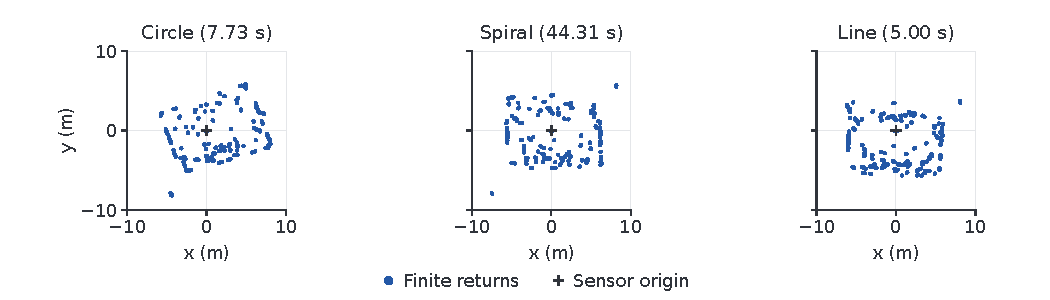
\includegraphics[width=7.0in]{figures/lidar_results.pdf}
  \caption{Midpoint LiDAR scans in their individual sensor frames; $+$ marks the sensor origin. Times are relative to each LiDAR log's first timestamp.}
  \label{fig:lidar}
\end{figure}

\noindent\begin{minipage}[t]{0.49\textwidth}
  \vspace{0pt}
  \centering
  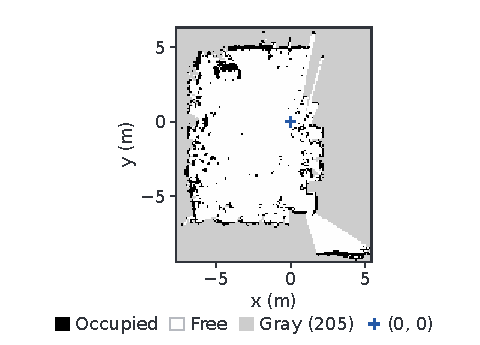
\includegraphics[width=3.2in]{figures/map_results.pdf}
  \captionof{figure}{Saved PGM map, 263$\times$315 cells at 0.05 m/cell. Lower-left origin: $(-7.72,-9.43)$ m, zero yaw.}
  \label{fig:map}
\end{minipage}\hfill
\begin{minipage}[t]{0.48\textwidth}
  \vspace{2pt}
  \raggedright
  Figure~\ref{fig:map} preserves the saved map's pixels.
  A broad free region and room boundary are visible, but scattered returns and thick, broken boundaries limit geometric precision.
  Grey unknown/intermediate cells occupy 49.3\% of the image.
  The YAML free threshold, 0.25, exceeds grey-205 occupancy $50/255\approx0.196$, so these cells would reload as free; this metadata limitation requires correction before reuse.
\end{minipage}
